%==============================================================================
% tento soubor pouzijte jako zaklad
% this file should be used as a base for the thesis
% (c) 2008 Michal Bidlo
% E-mail: bidlom AT fit vutbr cz
% Šablonu upravil / template edited by: Ing. Jaroslav Dytrych, dytrych@fit.vutbr.cz
%==============================================================================
% kodovaní: UTF-8 (zmena prikazem iconv, recode nebo cstocs)
% encoding: UTF-8 (you can change it by command iconv, recode or cstocs)
%------------------------------------------------------------------------------
% zpracování / processing: make, make pdf, make clean
%==============================================================================
% Soubory, které je nutné upravit: / Files which have to be edited:
%   projekt-20-literatura-bibliography.bib - literatura / bibliography
%   projekt-01-kapitoly-chapters.tex - obsah práce / the thesis content
%   projekt-30-prilohy-appendices.tex - přílohy / appendices
%==============================================================================
%\documentclass[]{fitthesis} % bez zadání - pro začátek práce, aby nebyl problém s překladem
\documentclass[english]{fitthesis} % without assignment - for the work start to avoid compilation problem
%\documentclass[zadani]{fitthesis} % odevzdani do wisu - odkazy jsou barevné
%\documentclass[english,zadani]{fitthesis} % for submission to the IS FIT - links are color
%\documentclass[zadani,print]{fitthesis} % pro tisk - odkazy jsou černé
%\documentclass[english,zadani,print]{fitthesis} % for the print - links are black
% * Je-li prace psana v anglickem jazyce, je zapotrebi u tridy pouzit
%   parametr english nasledovne:
%   If thesis is written in english, it is necessary to use
%   parameter english as follows:
%      \documentclass[english]{fitthesis}
% * Je-li prace psana ve slovenskem jazyce, je zapotrebi u tridy pouzit
%   parametr slovak nasledovne:
%      \documentclass[slovak]{fitthesis}

% Základní balíčky jsou dole v souboru šablony fitthesis.cls
% Basic packages are at the bottom of template file fitthesis.cls
%zde muzeme vlozit vlastni balicky / you can place own packages here

%---rm---------------
\renewcommand{\rmdefault}{lmr}%zavede Latin Modern Roman jako rm / set Latin Modern Roman as rm
%---sf---------------
\renewcommand{\sfdefault}{qhv}%zavede TeX Gyre Heros jako sf
%---tt------------
\renewcommand{\ttdefault}{lmtt}% zavede Latin Modern tt jako tt

% vypne funkci šablony, která automaticky nahrazuje uvozovky,
% aby nebyly prováděny nevhodné náhrady v popisech API apod.
% disables function of the template which replaces quotation marks
% to avoid unnecessary replacements in the API descriptions etc.
\csdoublequotesoff

% =======================================================================
% balíček "hyperref" vytváří klikací odkazy v pdf, pokud tedy použijeme pdflatex
% problém je, že balíček hyperref musí být uveden jako poslední, takže nemůže
% být v šabloně
% "hyperref" package create clickable links in pdf if you are using pdflatex.
% Problem is that this package have to be introduced as the last one so it
% can not be placed in the template file.
\ifWis
\ifx\pdfoutput\undefined % nejedeme pod pdflatexem / we are not using pdflatex
\else
  \usepackage{color}
  \usepackage[unicode,colorlinks,hyperindex,plainpages=false,pdftex]{hyperref}
  \definecolor{links}{rgb}{0.4,0.5,0}
  \definecolor{anchors}{rgb}{1,0,0}
  \def\AnchorColor{anchors}
  \def\LinkColor{links}
  \def\pdfBorderAttrs{/Border [0 0 0] }  % bez okrajů kolem odkazů / without margins around links
  \pdfcompresslevel=9
\fi
\else % pro tisk budou odkazy, na které se dá klikat, černé / for the print clickable links will be black
\ifx\pdfoutput\undefined % nejedeme pod pdflatexem / we are not using pdflatex
\else
  \usepackage{color}
  \usepackage[unicode,colorlinks,hyperindex,plainpages=false,pdftex,urlcolor=black,linkcolor=black,citecolor=black]{hyperref}
  \definecolor{links}{rgb}{0,0,0}
  \definecolor{anchors}{rgb}{0,0,0}
  \def\AnchorColor{anchors}
  \def\LinkColor{links}
  \def\pdfBorderAttrs{/Border [0 0 0] } % bez okrajů kolem odkazů / without margins around links
  \pdfcompresslevel=9
\fi
% * <nogikdeveloper@gmail.com> 2017-02-09T08:44:07.365Z:
%
% ^.
\fi
% Řešení problému, kdy klikací odkazy na obrázky vedou za obrázek
% This solves the problems with links which leads after the picture


\usepackage[all]{hypcap}
\usepackage{amsmath}
\usepackage[numbers,sort]{natbib}
\newenvironment{conditions}[1][kde:]
  {\begin{minipage}{\textwidth}
   \vspace*{-.5\belowdisplayskip}%
   \linespread{1}\selectfont #1 \begin{tabular}[t]{>{$}l<{$} @{${}:{}$} l}}
  {\end{tabular}\end{minipage}\\[\belowdisplayskip]}

\newenvironment{conditions*}[1][kde:]
  {\begin{minipage}{\textwidth}
   \vspace*{-.5\belowdisplayskip}%
   \linespread{1}\selectfont #1 \begin{tabular}[t]{>{$}l<{$} @{}>{${}}c<{{}$}@{} l}}
  {\end{tabular}\end{minipage}\\[\belowdisplayskip]}


\newcommand{\norm}[1]{\left\lVert #1 \right\rVert}

% Informace o práci/projektu / Information about the thesis
%---------------------------------------------------------------------------
\projectinfo{
  %Prace / Thesis
  project=SP,            %typ prace BP/SP/DP/DR  / thesis type (SP = term project)
  year=2019,             %rok odevzdání / year of submission
  date=\today,           %datum odevzdani / submission date
  %Nazev prace / thesis title
  title.cs={Deskriptor pro identifikaci osoby podle\\obličeje},  %nazev prace v cestine ci slovenstine (dle zadani) / thesis title in czech language (according to assignment)
  title.en={Descriptor for Identification of a Person by the Face}, %nazev prace v anglictine / thesis title in english
  %Autor / Author
  author={Tomáš Coufal},   %cele jmeno a prijmeni autora / full name and surname of the author
  author.name={Tomáš},     %jmeno autora (pro citaci) / author name (for reference)
  author.surname={Coufal}, %prijmeni autora (pro citaci) / author surname (for reference)
  author.title.p={Bc.},      %titul pred jmenem (nepovinne) / title before the name (optional)
  %author.title.a=PhD,     %titul za jmenem (nepovinne) / title after the name (optional)
  %Ustav / Department
  department=UITS, % doplnte prislusnou zkratku dle ustavu na zadani: UPSY/UIFS/UITS/UPGM
  %                  fill in appropriate abbreviation of the department according to assignment: UPSY/UIFS/UITS/UPGM
  %Skolitel / supervisor
  supervisor=Tomáš Goldmann, %cele jmeno a prijmeni skolitele / full name and surname of the supervisor
  supervisor.name={Tomáš},   %jmeno skolitele (pro citaci) / supervisor name (for reference)
  supervisor.surname={Goldmann},   %prijmeni skolitele (pro citaci) / supervisor surname (for reference)
  supervisor.title.p={Ing.},   %titul pred jmenem (nepovinne) / title before the name (optional)
  %supervisor.title.a={Ph.D.},    %titul za jmenem (nepovinne) / title after the name (optional)
  %Klicova slova, abstrakty, prohlaseni a podekovani je mozne definovat
  %bud pomoci nasledujicich parametru nebo pomoci vyhrazenych maker (viz dale)
  %Keywords, abstracts, declaration and acknowledgement can be defined by following
  %parameters or using dedicated macros (see below)
  %===========================================================================
  %Klicova slova / keywords
  %keywords.cs={Klíčová slova v českém jazyce.}, %klicova slova v ceskem ci slovenskem jazyce
  %                                              keywords in czech or slovak language
  %keywords.en={Klíčová slova v anglickém jazyce.}, %klicova slova v anglickem jazyce / keywords in english
  %Abstract
  %abstract.cs={Výtah (abstrakt) práce v českém jazyce.}, % abstrakt v ceskem ci slovenskem jazyce
  %                                                         abstract in czech or slovak language
  %abstract.en={Výtah (abstrakt) práce v anglickém jazyce.}, % abstrakt v anglickem jazyce / abstract in english
  %Prohlaseni / Declaration
  %declaration={Prohlašuji, že jsem tuto bakalářskou práci vypracoval samostatně pod vedením pana ...},
  %Podekovani (nepovinne) / Acknowledgement (optional)
  %acknowledgment={Zde je možné uvést poděkování vedoucímu práce a těm, kteří poskytli odbornou pomoc.} % nepovinne
  %acknowledgment={Here it is possible to express thanks to the supervisor and to the people which provided professional help.} % optional
}

%Abstrakt (cesky, slovensky ci anglicky) / Abstract (in czech, slovak or english)
\abstract[cs]{Práce shrnuje dosavadní poznatky v oboru biometrie při řešení problematiky identifikace osoby podle tváře. Zaměřuje se na konvoluční neuronové sítě a kapsulové sítě. Dále se zabývá současnými, modernímy postupy a jejich praktickými implementacemi. V neposlední řadě nabízí vlastní implementaci obdobného řešení.}
\abstract[en]{Thesis provides an overview and discussion of current findings in the field of biometrics. In particular, their impact and evolution of solutions to human face recognition problem. Special attention is payed to convolutional neural networks and capsule networks. Thesis then lists current approaches and state-of-the-art implementations. Based on these findings it provides insight into engineering a very own solution.}

%Klicova slova (cesky, slovensky ci anglicky) / Keywords (in czech, slovak or english)
\keywords[cs]{obličej, rozpoznávání, identifikace, hlava, neuronové sítě, convolution, kapsule, CapsNet}
\keywords[en]{face, recognition, identification, head, neural network, convolution, capsules, CNN, CapsNet}

%Prohlaseni (u anglicky psane prace anglicky, u slovensky psane prace slovensky)
%Declaration (for thesis in english should be in english)
%\declaration{Prohlašuji, že jsem ....... vypracoval samostatně pod vedením pana .......
%Uvedl jsem všechny literární prameny a publikace, ze kterých jsem čerpal.}

% \declaration{Hereby I declare that this bachelor's thesis was prepared as an original author’s work under the supervision of Mr. X
% The supplementary information was provided by Mr. Y
% All the relevant information sources, which were used during preparation of this thesis, are properly cited and included in the list of references.}
\declaration{Hereby I declare that this masters's thesis was prepared as an original author’s work under the supervision of Mr.\ Ing.\ Tomáš Goldmann. All the relevant information sources, which were used during preparation of this thesis, are properly cited and included in the list of references.}

%Podekovani (nepovinne, nejlepe v jazyce prace) / Acknowledgement (optional, ideally in the language of the thesis)
\acknowledgment{}
%\acknowledgment{Here it is possible to express thanks to the supervisor and to the people which provided professional help
%(external submitter, consultant, etc.).}

% řeší první/poslední řádek odstavce na předchozí/následující stránce
% solves first/last row of the paragraph on the previous/next page
\clubpenalty=10000
\widowpenalty=10000
\usepackage{gensymb}
\usepackage{graphicx,subfigure}
\usepackage{enumitem}
\usepackage{siunitx}
\usepackage{todonotes}

\begin{document}
  % Vysazeni titulnich stran / Typesetting of the title pages
  % ----------------------------------------------
  \maketitle
  % Obsah
  % ----------------------------------------------
  \tableofcontents

  % Seznam obrazku a tabulek (pokud prace obsahuje velke mnozstvi obrazku, tak se to hodi)
  % List of figures and list of tables (if the thesis contains a lot of pictures, it is good)
\ifczech
  \renewcommand\listfigurename{Seznam obrázků}
\fi
\ifslovak
  \renewcommand\listfigurename{Zoznam obrázkov}
\fi

  % \listoffigures
\ifczech
  \renewcommand\listtablename{Seznam tabulek}
\fi
\ifslovak
  \renewcommand\listtablename{Zoznam tabuliek}
\fi

  % \listoftables

  % vynechani stranky v oboustrannem rezimu
  % Skip the page in the two-sided mode
  \iftwoside
    \cleardoublepage
  \fi

  % Text prace / Thesis text
  % ----------------------------------------------
  %=========================================================================

\chapter{Introduction}
\label{chapter:introduction}
It is essential to any living species to recognise others in their community. Evolution has allowed animals to develop many methods, how to identify fellow members. Different species use various senses to do so. Smell, vision or hearing are the most common ones. However, humankind relies mostly on their vision. We did not develop strong perception of smell or other senses, that we can utilise on purpose or over longer distances. Therefore we mostly use our vision.

Moreover our species developed a habit to cover ourselves in clothes, which left only certain parts of our body exposed. Usually that's head and hands. And since receptors for most of our senses are placed on head, we are required to have it exposed to be able to orient in surroundings. This makes the frontal part of our head, a face, a great candidate for identifying others\,\cite{history}. We can recognise many nuances of different elements on the face. Shape of eyes, nose or mouth, colour of our eyes\dots That's just a subset of all the available features we use.

In this era of computers and information technologies, mankind tend to use what we know and offload our skills and capabilities to artificial intelligence. We hope to sharpen and enhance our senses; obtain more knowledge or widen our possibilities. As an example, which is more deeply elaborated in this thesis, we are trying to "teach" machines to recognise faces in the same way as we do. And there are various reasons to do so.

\section{Motivation}
Facial recognition in computer science is used in many different ways. Some use cases require people to be recognised for personal or company security purposes, for surveillance or just for our convenience.

Automating security countermeasures is a huge driving factor. It allows us to devote our time to other activities then watching over our belongings. It ensures our privacy and well being of the community. Let's list some basic use cases:

\begin{itemize}
    \item \textbf{Personal security}: unlocking a smartphone or laptop, etc.
    \item \textbf{Enterprise security and state defence}: access control, customs and border control, etc.
    \item \textbf{Surveillance}: Outlaws identification in public places, riot control, etc.
\end{itemize}

Furthermore, automated recognition of people's faces and their identification can facilitate many other processes for our convenience. That usually means it can save us time and provide a better service. These use cases spans from face and smile detection on when focusing and timing a camera shot to automated tagging of individual's friend on social media networks.

\section{Justification}

As in any other field in computer science, there is an ongoing race to provide better service in facial recognition. There are multiple aspects used as a metric to define better solution and this varies for each use case. Once, it is essential to provide the best performing software, for automated recognition, in places where limited computational power is available. Other time, it is rather about precision and time required to recognise a face. Outrunning other solutions means better service and inventing new technologies along the way unlocks better understanding on our own thinking process. In this thesis the existing solutions will be elaborated in detail as well as principles used to achieve such results.

There are also different approaches used to create and design such solutions. Sometimes a naive approach is used, other times the implementation leverages different aspects of Artificial Intelligence, especially Neural Networks.

The aim of this thesis is to construct a very own solution to this problem, relying strictly on Neural Networks. Each part of the problem is explained and implemented. Comparison with existing solutions is offered as a part of the Available solutions chapter\,\ref{chapter:solutions}, later in this paper.


\section{Decomposition}

To recognise a human face is a complex problem. Therefore it is usually divided into smaller sub-tasks, which are easier to comprehend and solve. Firstly, it is required to understand the input data. This understanding provides means to fundamentally divide the problem into easily solvable sub-tasks. Let's define and describe what are the expectations and demands on the input, as well as elaborate the required outputs.

\subsection{In-the-wild pictures}

As wide as the use cases, the variety of input data is vast. Some cases depends on frontal pictures of faces, some accents the so-called \textit{in-the-wild} aspect. This is a term specifically used for pictures captured without cooperation of the subject. A person on the picture is usually captured from an angle, lacking eye contact and staged emotion, etc. This thesis aims to cover a topic of facial recognition over CCTV data. However it can be said that any in-the-wild pictures are suitable for this implementation. The sufficient resolution and recognizability is the most important feature and requirement on the input data. The model has to be able to find a face on the picture. Therefore even it the model would rely solely on CCTV data, the data feed has to provide enough detail of the person's face.

\begin{figure}[ht]
    \centering
    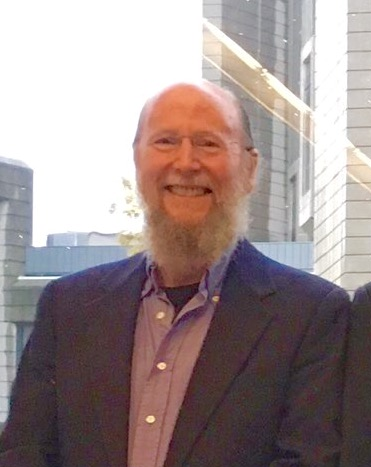
\includegraphics[height=15em]{obrazky-figures/richard_sutton.jpg}
    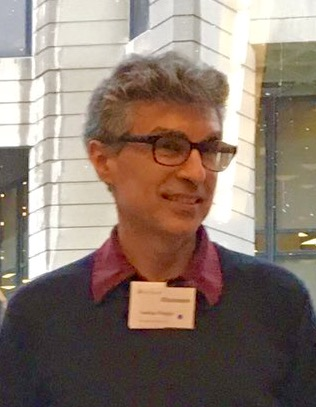
\includegraphics[height=15em]{obrazky-figures/yoshua_bengio.jpg}
    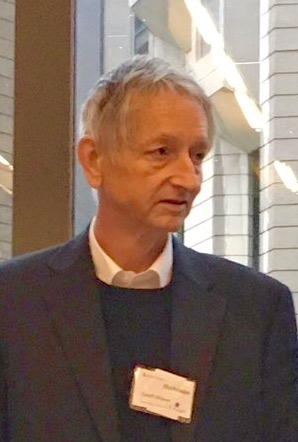
\includegraphics[height=15em]{obrazky-figures/geoffrey_hinton.jpg}
    \caption[Example of pictures in{-}the{-}wild]{Example of pictures in{-}the{-}wild. From left: Richard Sutton, Yoshua Bengio, Geoffrey Hinton. \textit{Source: Steve Jurvetson (CC BY 2.0\,\footnotemark)}}
\end{figure}

CCTV as a source of the input data has some crucial advantages for real world scenarios over any random pictures in-the-wild. Usually CCTV produces feeds, therefore the subject of recognition is captured on many frames of a video recording. That means, the model can be provided by many images of the same face and if properly configured and trained, it can leverage this aspect.

\subsection{Recognition and identification}
\footnotetext{\url{https://creativecommons.org/licenses/by/2.0/deed.en}}

Imagine an individual captured on a CCTV footage. To identify a person by face, we have to naturally focus the model on the face. Therefore the first step would be to detect where and if the picture captures a face. When such region is found, it is essential to detect all the facial features the models is trained to focus. Not always all features are available (the face can be partially covered, captured from an angle etc.)\,--\,the model has to adapt to such situation. Based on features detected, the model creates an normalised estimation of facial features. This normalised template should represent a frontal scan of facial features of the individual's face. When the model has access to multiple images of the face, it can produce multiple templates and combine them into one unique normalised master template, unique to the person.

\subsection{Output information}

Last but not least, let's define what is expected to be found in such pictures. A facial identification model aims to come up with a unique vector (face template) for each person. Unique in a sense of minimising inter-dimensionality and maximising intra-dimensionality. That means the vector extracted from a picture is similar to all other vectors for the same person, as much as possible. It is also the most different to vector assigned to other people. Naturally each picture of the same person can result into slightly different template. However this sample specific output vector is expected to be nearly identical to a summarised template for the person. This summarised template is a result of combining many output vectors for the same individual.


\chapter{Research and literature review}
\label{chapter:research}
\input{project-12-chapter-research}

\chapter{Available methods and models}
\label{chapter:methods}

\chapter{Discussion}
\label{chapter:discussion}


\chapter{Conclusion}
\label{chapter:conclusion}


%=========================================================================
 % viz. obsah.tex / see obsah.tex

  % Pouzita literatura / Bibliography
  % ----------------------------------------------
\ifslovak
  \makeatletter
  \def\@openbib@code{\addcontentsline{toc}{chapter}{Literatúra}}
  \makeatother
  \bibliographystyle{bib-styles/czechiso}
\else
  \ifczech
    \makeatletter
    \def\@openbib@code{\addcontentsline{toc}{chapter}{Literatura}}
    \makeatother
    \bibliographystyle{bib-styles/czechiso}
  \else
    \makeatletter
    \def\@openbib@code{\addcontentsline{toc}{chapter}{Bibliography}}
    \makeatother
    \bibliographystyle{bib-styles/englishiso}
  %  \bibliographystyle{alpha}
  \fi
\fi
  \begin{flushleft}
  \bibliography{project-20-bibliography}
  \end{flushleft}

  % vynechani stranky v oboustrannem rezimu
  % Skip the page in the two-sided mode
  \iftwoside
    \cleardoublepage
  \fi

  % Prilohy / Appendices
  % ---------------------------------------------
  \appendix
\ifczech
  \renewcommand{\appendixpagename}{Přílohy}
  \renewcommand{\appendixtocname}{Přílohy}
  \renewcommand{\appendixname}{Příloha}
\fi
\ifslovak
  \renewcommand{\appendixpagename}{Prílohy}
  \renewcommand{\appendixtocname}{Prílohy}
  \renewcommand{\appendixname}{Príloha}
\fi
  \appendixpage

% vynechani stranky v oboustrannem rezimu
% Skip the page in the two-sided mode
\iftwoside
  \cleardoublepage
\fi

\ifslovak
%  \section*{Zoznam príloh}
%  \addcontentsline{toc}{section}{Zoznam príloh}
\else
  \ifczech
%    \section*{Seznam příloh}
%    \addcontentsline{toc}{section}{Seznam příloh}
  \else
%    \section*{List of Appendices}
%    \addcontentsline{toc}{section}{List of Appendices}
  \fi
\fi
  \startcontents[chapters]
  % seznam příloh / list of appendices
  % \printcontents[chapters]{l}{0}{\setcounter{tocdepth}{2}}

  % vynechani stranky v oboustrannem rezimu
  \iftwoside
    \cleardoublepage
  \fi
  \chapter{CD Content}

\begin{itemize}
    \item \texttt{src}: Source codes for \texttt{CapsNet} package.
    \item \texttt{src/notebooks}: Example \textit{Jupyter} notebooks for training and testing a model.
    \item \texttt{src/saved\_models}: Saved models ready to be imported and used.
    \item \texttt{src/README.md}: Installation and usage manual.
    \item \texttt{thesis}: Source codes to build this thesis PDF.
    \item \texttt{thesis.pdf}: This very same thesis as a PDF file.
\end{itemize}
 % viz. prilohy.tex / see prilohy.tex
\end{document}
